% !TeX root = ../main.tex
\chapter{回环检测}
我们之前介绍了前端视觉里程计和后端优化,前端提供了特征点的提取和轨迹、地图的初值,而后端则对这些数据进行优化,但是如果我们前端提取的数据本来就有问题,久而久之,后端的优化还是会出问题。所以,这个时候我们就需要提供一些时隔更加久远的约束,例如回环检测。
\par
\begin{figure}[H]
	\centering
	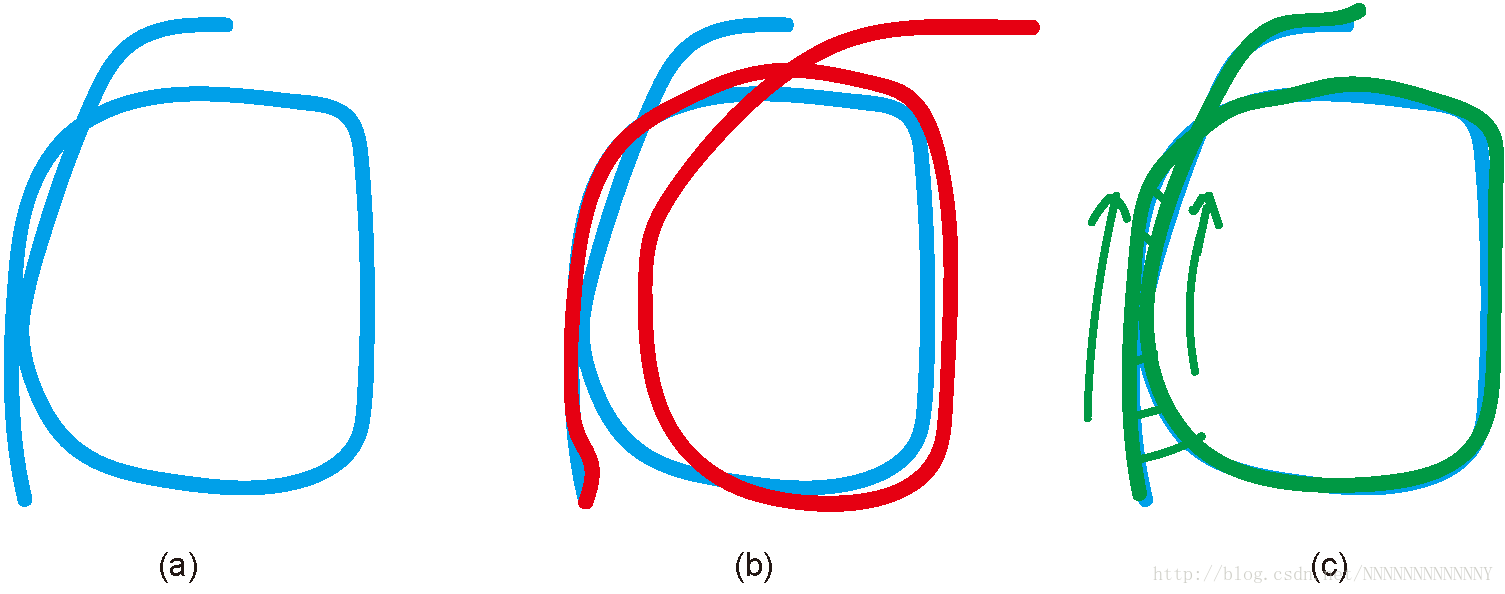
\includegraphics[height=5cm]{loopdetection}
	\caption{回环检测作用}
\end{figure}
而回环检测的关键就是如何有效检测出摄像头经过同一个地方这件事。如果我们能检测到这一事实,就能为后端优化提供更多信息,使之能够得到一个更好的轨迹估计。\par
回环检测对于SLAM系统意义重大,关系到我们的系统估计的轨迹长时间下的正确性。另一方面,由于回环检测提供了当前数据与所有历史数据的关联,在跟踪算法丢失后,我们还可以利用回环检测进行重定位。所以,回环检测对于整个SLAM系统的鲁棒性的提升是非常明显的。
\section{回环检测方法}
最简单的检测回环检测的方式就是让所有新来的关键帧对之前的关键帧都做一遍特征匹配,根据正确匹配的数量确定哪两幅图像存在关联。这个思想确实有效,但是这个思想会导致我们检测的数量过大。另一种思想就是随机抽取图像进行比较,但是这样时间一长,系统能判断回环的概率会大大降低,使得检测效率不高。\par
上面说的两中方法都过于简单,但有一点是可以肯定的,为了进行回环检测,我们主要进行的工作就是比较两幅图片,那么核心问题就是如何计算图像间的相似性。比如,对于图像A和图像B,我们要设计一种方法计算两幅图像的相似性:$S(A, B)$。
\section{模型的评判标准}
在统计学中,一个检测模型的好坏主要是计算两个统计量:准确率(Precision)和召回率(Recall)。
\begin{table}[H]
	\centering
	\caption{混淆矩阵}
	\label{hunxiaojuzhen}
\begin{tabular}{|l|cc|}
	\hline
	\diagbox{预测}{事实} & 是回环 & 不是回环\\
	\hline
	是回环 & 真阳性(TP) & 假阳性(FP) \\
	不是回环 & 假阴性(FN) & 真阴性(TN) \\
	\hline
\end{tabular}
\end{table}
按照表\ref{hunxiaojuzhen}所述,公式如下:
\begin{equation}
Precision=\frac{\mathrm{TP}}{\mathrm{TP}+\mathrm{FP}}\\
Recall=\frac{\mathrm{TP}}{\mathrm{TP}+\mathrm{FN}}\\
\end{equation}
从公式上来看,准确率描述的是算法提取的所有回环中确实是真实回环的概率;而召回率则是说在所有真实回环中被正确检测出的概率。\par
在一个SLAM系统中,准确率更为重要,而召回率则能宽容一点。这是因为如果我们错将所有的椅子当成同一张,那么将这些数据传入后端优化,我们就能看到走廊不直了,墙壁交错,整张地图都失效了。而相比之下,召回率低一点,则顶多有部分的回环没有被检测到,地图可能会受一点累计误差的影响,然而这些误差只需要一两次回环就能完全消除了。所以在选择回环检测算法时,我们更倾向与将参数设置得更为严格,或者在检测之后再加上回环验证的步骤。\par
\section{模型设计}
那么直观上看,图像能表示成矩阵的形式,如果我们直接让两幅图像相减,这样计算图像相似性如何呢?事实上经过实验我们会发现这个方法的准确率和召回率都很差,这是因为两张相同场景的图像,他们的光照,角度等信息可能都不一样,所以这种直接相减的方法很难有好的结果。下面我们来介绍一下词袋模型。
\subsection{词袋模型}
\subsubsection{模型概述}
既然直接用两幅图像相减的方式不好,那么我们可以像前端视觉里程计那样对两幅图像的特征点来做回环检测,只要匹配数量大于一定值,就认为出现了回环。\par
词袋,也就是Bag-of-Words(BoW),目的是用“图像上的几种特征”来描述一副图像。例如我们说某张图像中有两个人、三张椅子;而另一幅图像中有一个人、一张桌子。那么根据这样的描述我们就可以度量这两幅图像的相似性。再具体一些,我们只要做以下的事情:
\begin{enumerate}
\item 确定“人”、“桌子”、“椅子”等概念——对应BoW中的单词(Words),许多单词放在一起,组成了“字典”。
\item 确定一副图像中出现了哪些字典中定义的概念——我们用单词出现的情况来描述整幅图像。这样就把一副图像转为一个向量的描述。
\item 比较上一步中的描述的相似程度。从上面的例子来说,首先我们要通过某种方式获得一本“字典”。字典上记录的是我们定义的单词,每个单词都有一定意义。然后我们定义一个向量,这个向量描述的就是这幅图像出现在字典上的物体数量。
\end{enumerate}

这样我们就能根据一个向量描述一副图像了,这个相邻描述的是“图像是否含有某类特征”的信息,比单纯的灰度值更加稳定。这里强调的是物体的有无而与物体的空间排列顺序有关。
6.2.2 字典的结构	
根据我们上面的描述,我们可以看出字典由许多单词组成,而每一个单词代表了一个概念。与特征点不同,一个单词不是从单幅图像上提取出来的,而是某一类特征的组合。所以,字典生成的问题类似于机器学习中聚类的问题。
聚类问题在无监督机器学习中非常常见,用于让极其自行寻找数据中的规律。首先,假设我们对大量的图像提取了特征点,比如说有N个。那么如果我们想创建一个有k个单词的字典,每个单词都可以看作是局部相邻特征点的集合。我们应该使用经典的K-means算法解决,具体方法如下:
(1)随机选取k个中心点:。
(2)对每一个样本,计算它与每个中心点之间的距离,取最小的作为它的归类。
(3)重新计算每个类的中心点。
(4)如果每个中心点都变化很小,则算法收敛,退出;否则返回第二步。
在BoW中,我们通常会使用一个较大规模的字典,以保证当前使用环境中的图像特征都曾在字典中出现,或至少有相近的表现。那么我们在寻找单词的时候,也是有的复杂度。那么我们如果使用二分查找显然可以提升查找效率,打到对数级别的复杂度。在本文中,我们使用k叉树来表达字典。假如我们希望构建一个深度为d、每次分叉为k的树,那么做法如下:
(1)在根节点,用k-means把所有样本聚成k类,这样就得到了第一层。
(2)对第一层的每个节点,把属于该节点的样本再聚成k,得到下一层。
(3)以此类推,最后得到叶子层。叶子层便是所谓的Words。
最后,我们仍在叶子层构建了单词,而树结构中的中间节点仅供快速查找使用。这样一个k分支、深度为d的树,可以容纳个单词。另一方面,我们如果要查找一个单词,只需比较中间节点的聚类中心比较(一共d次),即可找到最后的单词,保证了对数级别的查找效率。
6.2.3 相似度计算
在建立了字典之后,我们只要在字典树中逐层查找,最后都能找到与之对应的单词,这样我们就需要来判断图像的相似性问题了。在文本检索中,常用的一种做法称为TF-IDF。TF部分的思想是,某单词在一副图像中经常出现,它的区分度就高。IDF的思想是,某单词在字典中出现的频率也高,那么分类图像时区分度越高。
在词袋模型中,在建立字典时可以考虑IDF部分。我们统计某个叶子节点中的特征数量相对于所有特征数量的比例作为IDF部分。假设所有特征数量为n,数量为,那么该单词的IDF为:

另一方面,TF部分则是指某个特征在某幅图像中出现的频率。假设图像A中单词出现了次,而一共出现的单词次数为n,那么TF为:

那么的权重等于TF乘IDF之积。
